\documentclass{homework}

\title{Homework 1}
\author{Kevin Evans}
\studentid{11571810}
\date{August 31, 2021}
\setclass{Math}{364}
\usepackage{amssymb}
\usepackage{mathtools}
\usepackage{graphicx}
\usepackage{amsthm}
\usepackage{amsmath}
\usepackage{slashed}
\usepackage{boldline}
\usepackage{physics}
\usepackage{tcolorbox}
\usepackage[inter-unit-product =\cdot]{siunitx}

\usepackage[makeroom]{cancel}
\usepackage{booktabs}

\usepackage{times}
\usepackage{mhchem}

%\usepackage{calligra}
%\DeclareMathAlphabet{\mathcalligra}{T1}{calligra}{m}{n}
%\DeclareFontShape{T1}{calligra}{m}{n}{<->s*[2.2]callig15}{}
%\newcommand{\scriptr}{\mathcalligra{r}\,}
%\newcommand{\boldscriptr}{\pmb{\mathcalligra{r}}\,}
%\newcommand{\emf}{\mathcal{E}}
\newcommand{\st}{\mathrm{s.t.}}
\begin{document}
	\maketitle
	\begin{enumerate}
		\item[2.2.8] \underline{Problem}.\quad Premium loam is 60\% soil and 40\% domestic manure and costs \$5/50 lb. Generic loam is 20\% soil and 10\% domestic manure (and 70\% sand, stone, etc.) and costs \$1/50 lb. We need loam for our backyard that is at least 36\% soil and at least 20\% domestic manure. What combination of the two loams should we use to minimize costs?
		
		\textit{Solution}.\quad First, we'll need to identify the decision variables. The practical choice seems to be how much of each loam do we need, \begin{align*}
			\text{Let } x & = \text{pounds of premium loam}, \\
			y & = \text{pounds of generic loam}.
		\end{align*}
		Next, we can identify the objective function. Since the problem requires the cost to be minimized, \begin{align*}
			\text{Let } z & = \text{cost of both loams in dollars} \\
				& = 5 x / 50 + y / 50\\
				& = 0.10x + 0.02y
		\end{align*}
		Finally, we can identify the constraints using the requirements of the loam and composition of each. For this, I'm assuming we'll need 100 lbs total of loam, then we'll need at least 36 lbs of soil and 20 lbs manure. \begin{align*}
			100 & = x + y \\
			36 & \le 0.60x + 0.20y \\
			20 & \le 0.40x + 0.10y \\
			x, y & \ge 0 \\
			x, y & \in \mathbb{R}
		\end{align*}
		Combining this, the linear program is 
		\begin{tcolorbox}
			\vspace{-1em}
			\begin{align*}
				\min_{x, y \: \in \: \mathbb{R}} \quad z & = 0.10x + 0.02 y  \\
				\st \quad 
				100 & = x + y \\
				36  & \le 0.60 x + 0.20y \\
				20 & \le 0.40 x + 0.10y \\
				x, y & \ge 0
			\end{align*}
		\end{tcolorbox}
		Plotting the constraints in Desmos (on next page), the vertex that intersects the 100 lb constraint in the feasible region is $(x^*, y^*) = (40, 60)$. The \textbf{cost is minimized when we use 40\% premium loam and 60\% generic loam}, with a cost of $z^*=$ \$5.20/100 lbs.
		
		\begin{center}
			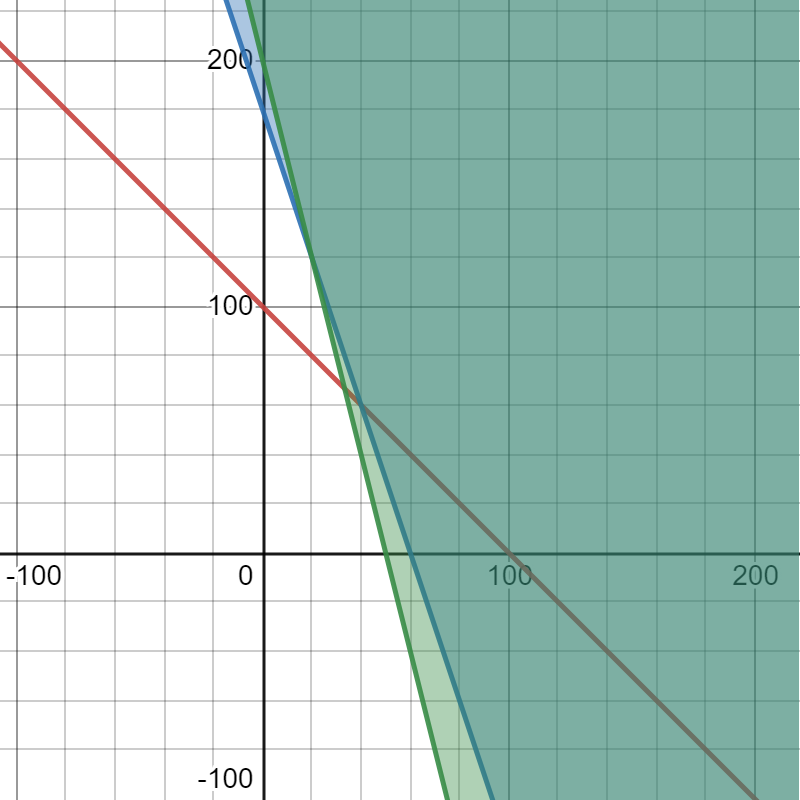
\includegraphics[width=0.7\linewidth]{screenshot001}
		\end{center}
		
		
		\pagebreak
		
		\item[2.2.13] \underline{Problem}. A coin is to be minted containing at least 40\% silver and at least 50\% copper. The mint has available alloys A, B, C, and D, with the following compositions and costs:
		
		\begin{center}
			\begin{tabular}{lcccc}
				\toprule
				& A & B & C & D \\
				\midrule
				\textit{\% Silver} & 30 & 35 & 50 & 40 \\
				\textit{\% Copper} & 60 & 35 & 50 & 45 \\
				\textit{Cost/lb (\$)} & 11 & 12 & 16 & 14 \\
				\bottomrule
			\end{tabular}
		\end{center}
		What blend of these alloys provide the required composition at minimal cost?
		
		\textit{Solution.} The decision variables can be the weight of each alloy, \begin{align*}
			\text{Let } x_k & = \text{the weight in pounds of the $k$th alloy}.
		\end{align*}
		Since the cost is minimized, the total cost will be the objective function, \begin{align*}
			\text{Let } z & = c^T x
			\intertext{where $c$ is the cost in dollars associated with each alloy,}
			c & = \begin{pmatrix}
				11 & 12 & 16 & 14
			\end{pmatrix}.
		\end{align*}
		The constraints are given by the required alloys and the composition of each per 100 lbs, \begin{align*}
			\text{Let } A & = \text{the compositions of each alloy} \\
				& = \begin{pmatrix}
					1 & 30 & 60 \\
					1 & 35 & 35 \\
					1 & 50 & 50 \\
					1 & 40 & 45
				\end{pmatrix} \\
			\text{Let b } & = \text{the target blend of alloys} \\
				& = \begin{pmatrix}
					100 \\
					40 \\
					50
				\end{pmatrix}
		\end{align*}
		Combining these, the linear program can be given as
		\begin{tcolorbox}
			\vspace{-1em}
			\begin{align*}
				\min_{x \: \in \: \mathbb{R}^4} z & = c^T x & c & = \begin{pmatrix}
					11 & 12 & 16 & 14
				\end{pmatrix} \\
				A x & \ge b \\
				x & \ge 0  \\
				& & A & = \begin{pmatrix}
					1 & 30 & 60 \\
					1 & 35 & 35 \\
					1 & 50 & 50 \\
					1 & 40 & 45
				\end{pmatrix} \\
				& & b & = \begin{pmatrix}
					100 & 40 &  50
				\end{pmatrix}^T
			\end{align*}
		\end{tcolorbox}
	\end{enumerate}
\end{document}